\documentclass[
    a4paper
]{scrreprt}
\usepackage[ngerman]{babel}
\usepackage[utf8]{inputenc}
\usepackage{textcomp, expdlist, array, colortbl, xcolor}
\usepackage[pdftex]{graphicx}
\usepackage[TS1, T1]{fontenc}
\usepackage{palatino} % Schriftart
\usepackage{parskip} %Erste Zeile eines Paragrafen nicht einrücken

\usepackage{listings}
\usepackage{color}
\usepackage{xcolor}

\colorlet{punct}{red!60!black}
\definecolor{background}{HTML}{EEEEEE}
\definecolor{delim}{RGB}{20,105,176}
\colorlet{numb}{magenta!60!black}
\definecolor{mygreen}{rgb}{0,0.6,0}

\lstdefinelanguage{json}{
	basicstyle=\normalfont\ttfamily,
	stepnumber=1,
	numbersep=8pt,
	showstringspaces=false,
	breaklines=true,
	backgroundcolor=\color{background},
	morestring=[s][\color{red}]{"}{"},
	morekeywords={set, hash, key, list},
	morecomment=[l]{//},
	literate=
	*{0}{{{\color{numb}0}}}{1}
	{1}{{{\color{numb}1}}}{1}
	{2}{{{\color{numb}2}}}{1}
	{3}{{{\color{numb}3}}}{1}
	{4}{{{\color{numb}4}}}{1}
	{5}{{{\color{numb}5}}}{1}
	{6}{{{\color{numb}6}}}{1}
	{7}{{{\color{numb}7}}}{1}
	{8}{{{\color{numb}8}}}{1}
	{9}{{{\color{numb}9}}}{1}
	{:}{{{\color{punct}{:}}}}{1}
	{,}{{{\color{punct}{,}}}}{1}
	{\{}{{{\color{delim}{\{}}}}{1}
	{\}}{{{\color{delim}{\}}}}}{1}
	{[}{{{\color{delim}{[}}}}{1}
	{]}{{{\color{delim}{]}}}}{1}
	{1aba56d8c5}{{{\color{numb}1aba56d8c5}}}{10}
}

\lstset{
	language={json},
	commentstyle=\color{mygreen}
}


\begin{document}
    \sffamily % Whole document sans-serif


    % Titelseite
    \begin{titlepage}
        \centering
        
\includegraphics[width=0.8\textwidth]{./images/logo_hska.png}\par\vspace{1cm}
        \vspace{1cm}

        {\scshape\Large Verteile Systeme 2 -- Labor\par}
        \vspace{1.5cm}

        {\huge\textbf{Twitter-Klon}\par}
        \vspace{2cm}

        {\Large\itshape Timo Blust, 48594\par}
        {\Large\itshape Gennadi Eirich, 50629\par}
        {\Large\itshape Tim Essig, 49683\par}
        {\Large\itshape Maike Rees, 47307\par}

        \vfill

        % Bottom of the page
        {\large \today\par}
    \end{titlepage}


    % Inhaltsverzeichnis
    \tableofcontents


    % Aufgabe 1
    \chapter{Konzeption und Gestaltung}
    \section{Use Case Diagramm}
    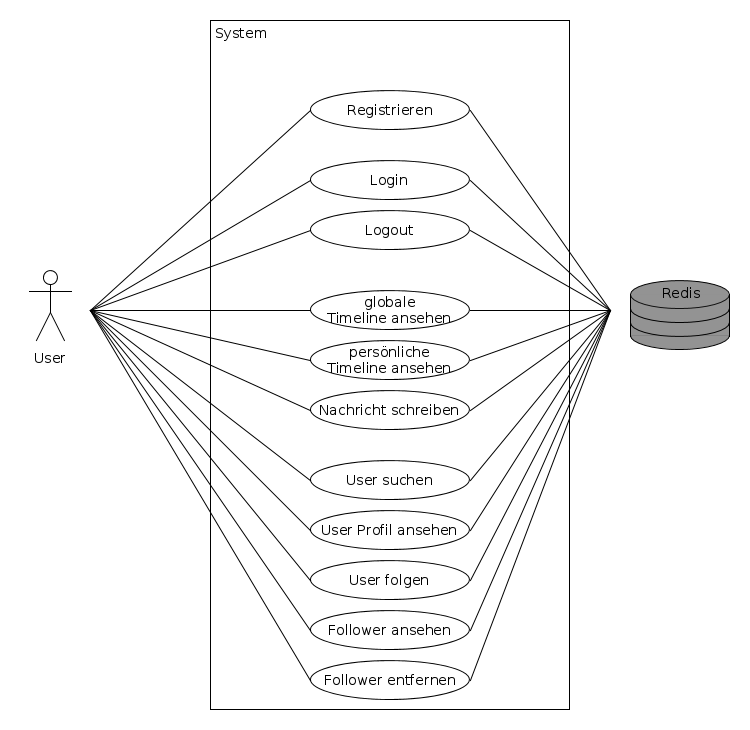
\includegraphics[width=\textwidth]{./images/useCaseDiagramm.png}

    \section{Entwurf der Seitennavigation}
	     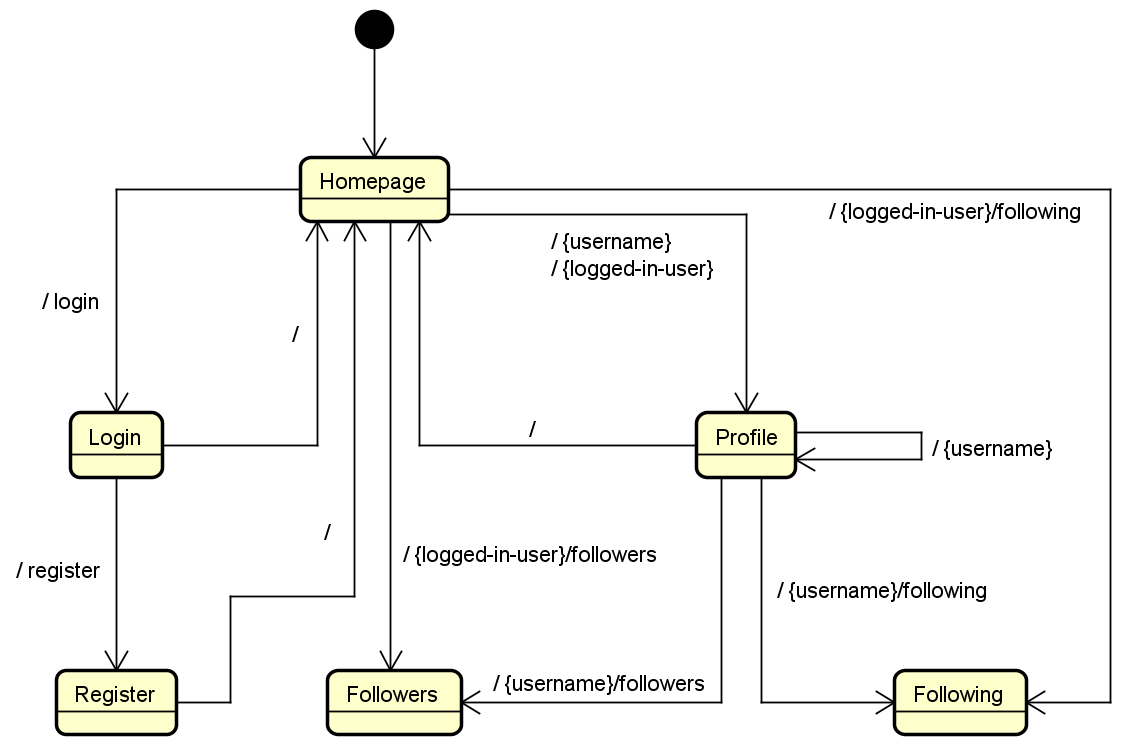
\includegraphics[width=\textwidth]{./images/state-machine.png}

    \section{Mockup}
		\includegraphics[width=\textwidth]{./images/1_login.png}
		Login\par\vspace{.6cm}
		\includegraphics[width=\textwidth]{./images/1_registration.png}
		Registration\par\vspace{.6cm}
		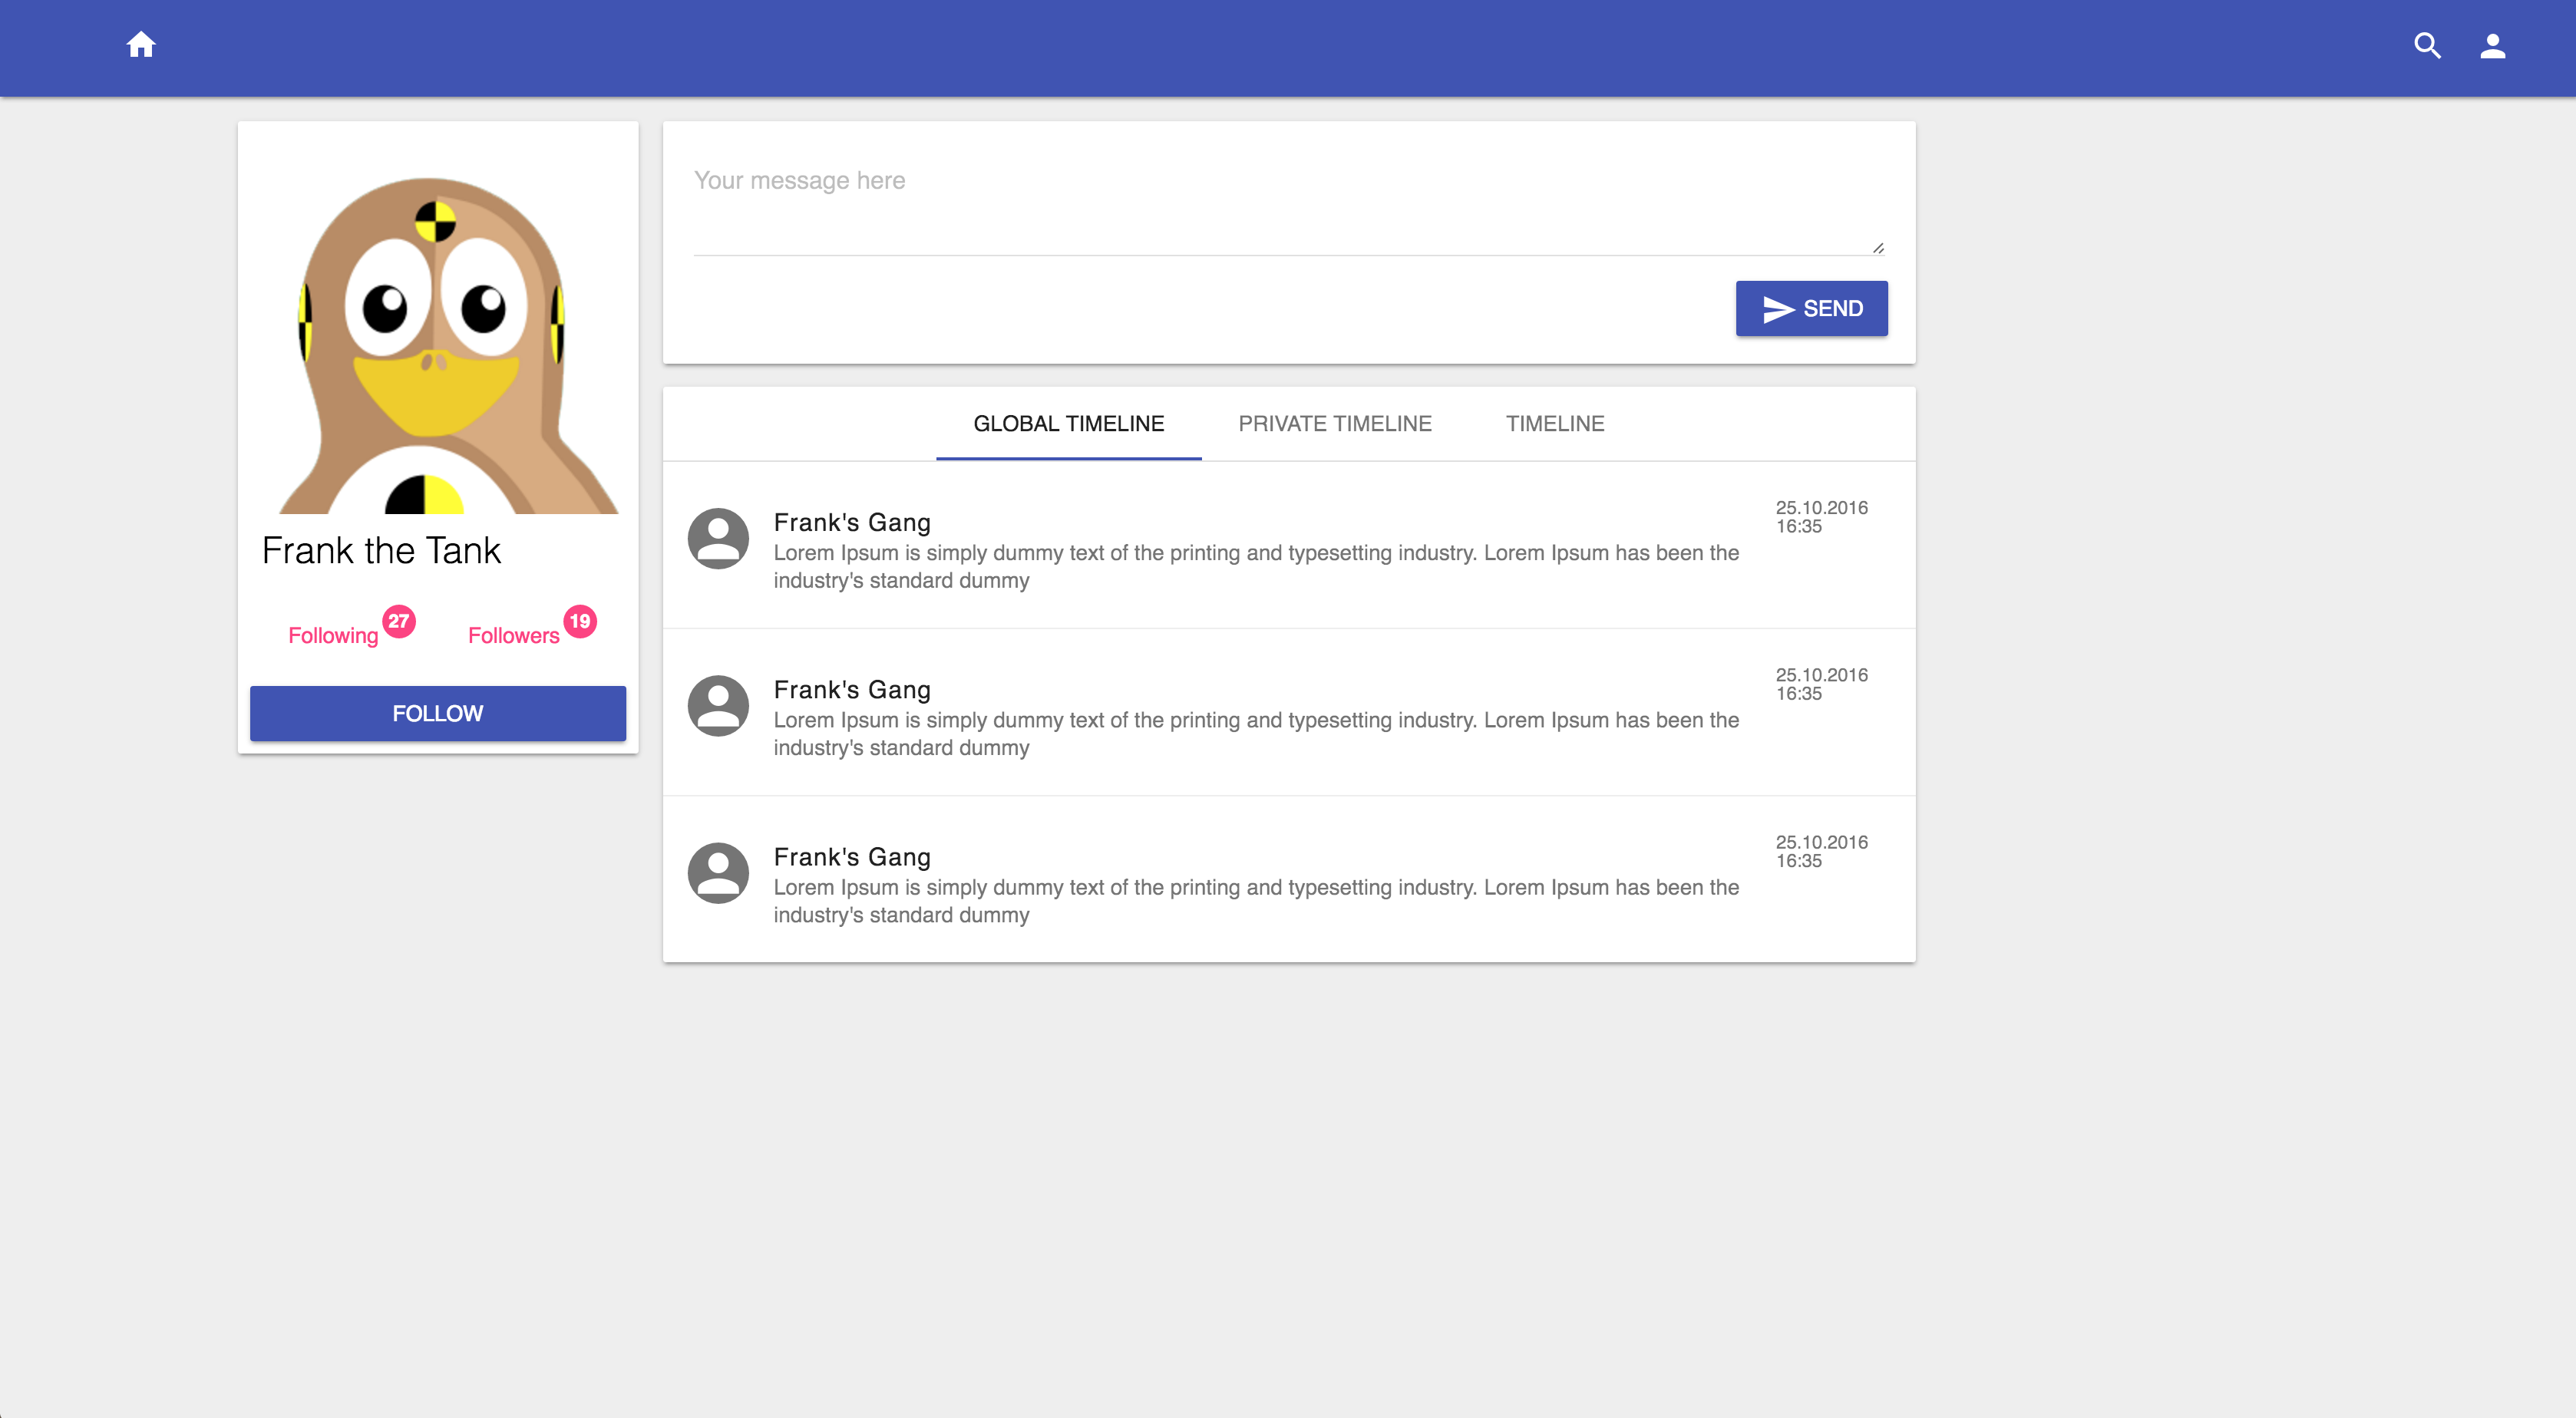
\includegraphics[width=\textwidth]{./images/1_home.png}
		Home\par\vspace{.6cm}
		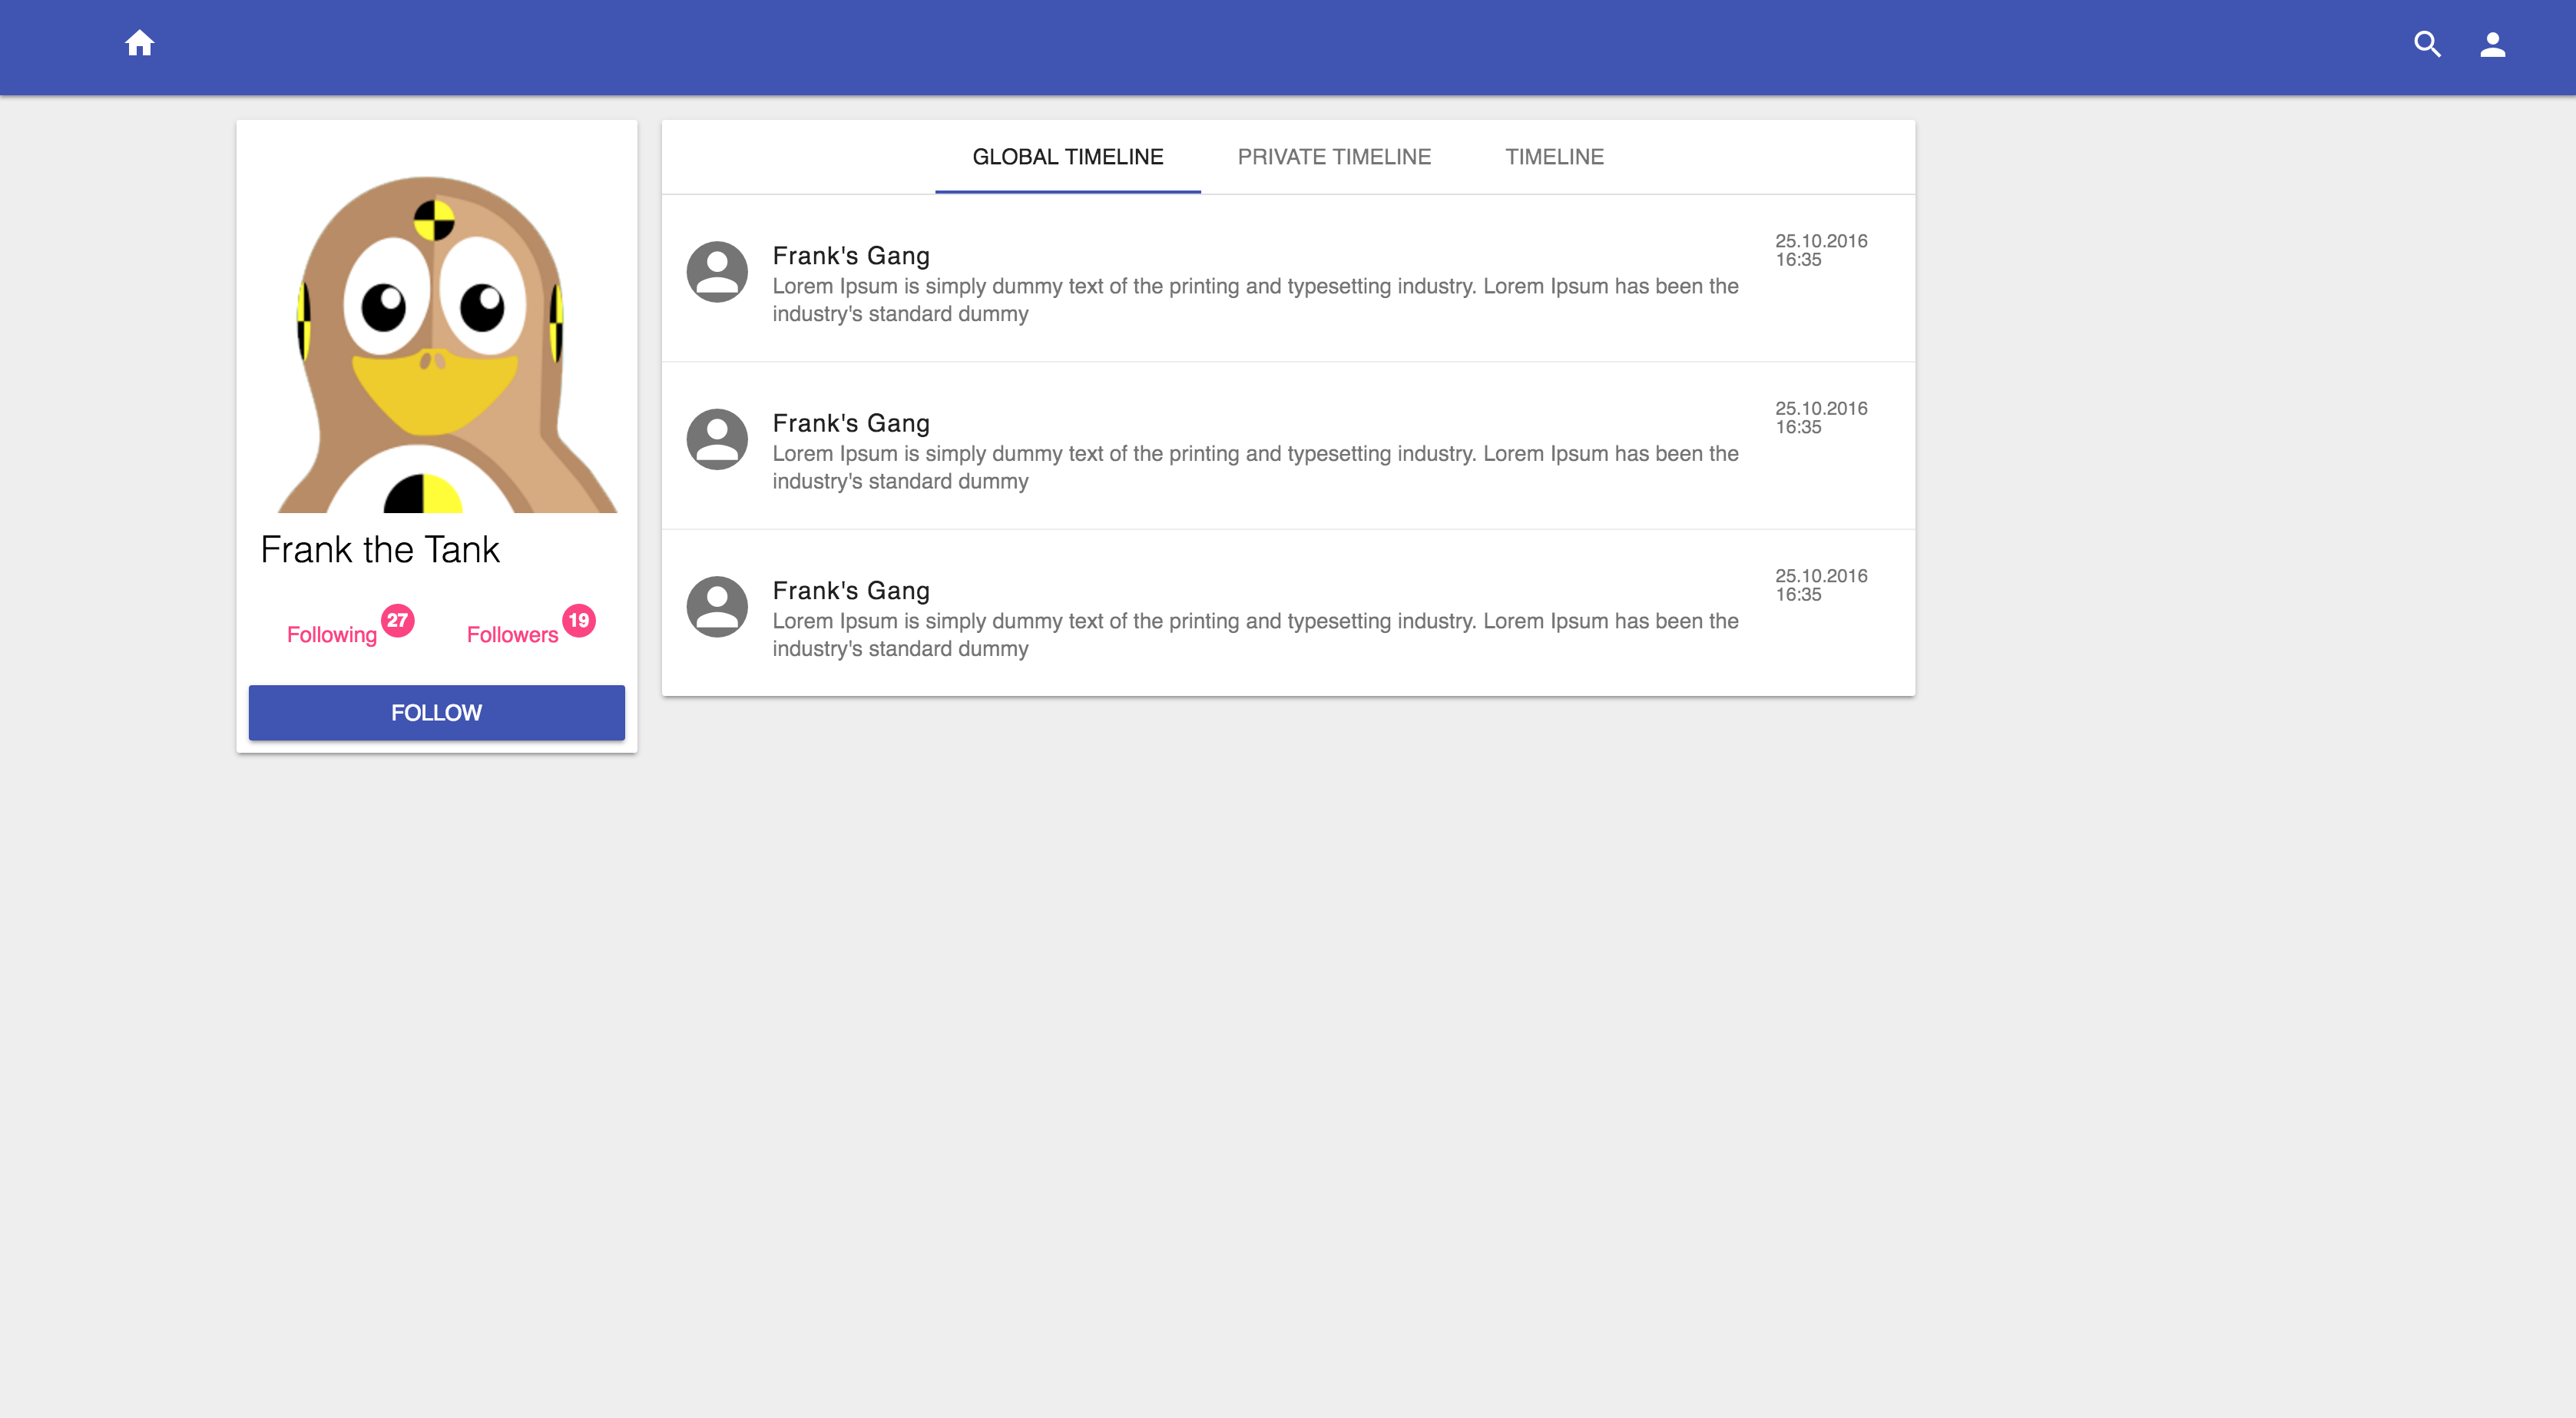
\includegraphics[width=\textwidth]{./images/1_user.png}
		Benutzeransicht\par\vspace{.6cm}
		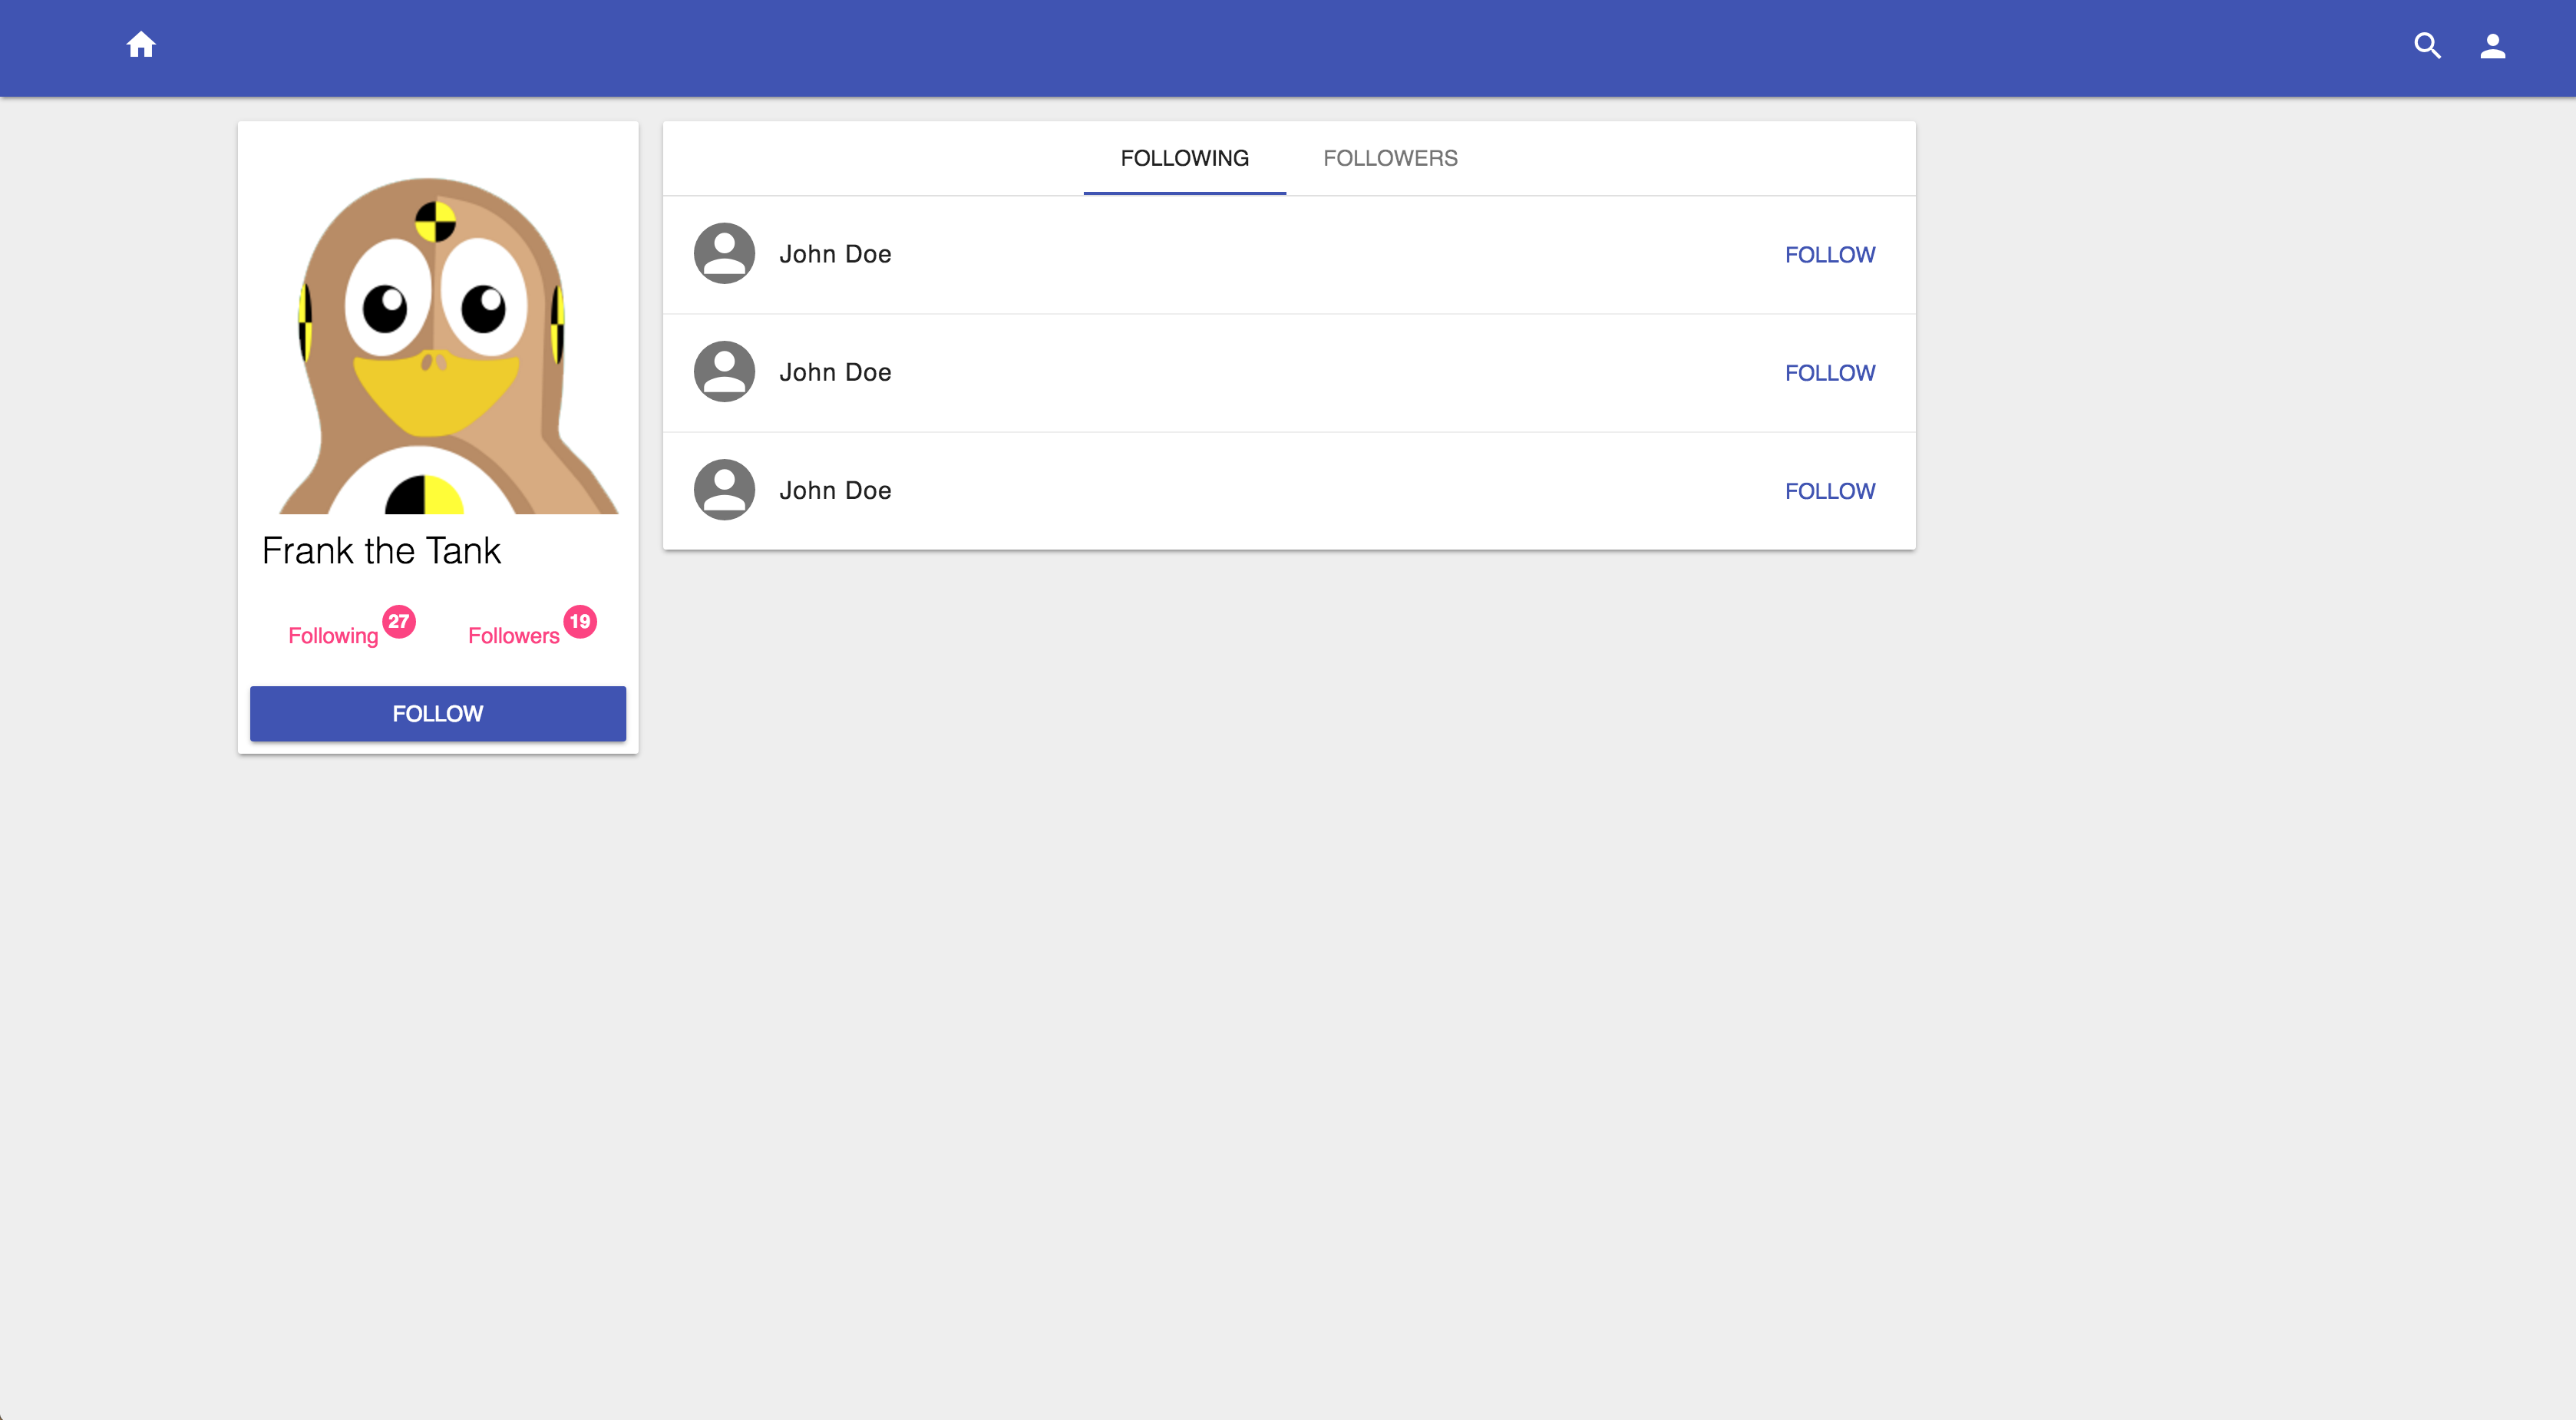
\includegraphics[width=\textwidth]{./images/1_user_followers.png}
		Followerliste des Benutzers

    \section{Datenmodell}
        \begin{lstlisting}[language=json]
//Set aller User
set user:all = {"essigt", "eirichg", "reesm", "blustt"}

//HashSets fuer die einzelnen Nutzer
hash user:*
    user:essigt = {id: "1", username: "essigt", firstname: "Tim", lastname: "Essig", password: "xyz", auth: "1aba56d8c5"}

//Sets um zu speichern, wer wem folgt
set user:*:follower
set user:*:following

//Keys um einen auth-token einem username zuzuordnen
key auth:*:username
    auth:1aba56d8c5:username = essigt

//Liste aller Posts
list post:all = {1,2,3,4}

//HashSets fuer die einzelnen Posts
hash post:*
    post:1 = {timestamp: 01-03-2016 13:37, message:"Meine tolle Nachricht", user:"essigt"}

list user:*:posts = {1} //Liste aller Posts eines Users
list timeline:* = {1,3} //Liste aller Posts der Follower des Users(incl. seiner eigenen)

//Globale Counter
key global:userid
key global:postid
        \end{lstlisting}


    % Aufgabe 2
    \chapter{Seitenbasierte Implementierung}
    \section{Redis Schnittstelle}

    \section{Sessionverwaltung}

    \section{MVC Implementierung}
    \subsection{Fronend}
	Um redundanten Code zu vermeiden, wurde die Templates in mehrere Fragment aufgeteilt. Thymeleaf bietet die Möglichkeit diese beim parsen einzubinden.
	
	Folgende Fragmente wurden erstellt:
	\begin{itemize} 
		\item Header
		\item Footer
		\item Profil/User
		\item Timeline
		\item Post
	\end{itemize}

	Auf jeder Seite, mit Ausnahme von \textbf{Login} und \textbf{Registrierung} werden die Komponente \textit{Header}, \textit{Footer} und \textit{Profil/User} eingebettet.
	
	In der Homepage und der Profilansicht wird zusätzlich die \textit{Timeline} eingebunden.\\
	
	\textbf{Beispiel: Profil/User - Fragment:}
	\begin{lstlisting}[language=html]
<div class="profile-card mdl-card mdl-shadow--2dp" th:fragment="card">
 <div id="profile-header" class="mdl-card__title">
  <h2 id="profile-name" class="mdl-card__title-text" th:text="${user.username}"></h2>
 </div>
		
 <div class="mdl-card__supporting-text">
  <a th:href="@{|/users/${user.username}/following|}" class="mdl-badge" th:attr="data-badge=${followingCnt}">Following</a>
  <a th:href="@{|/users/${user.username}/follower|}" class="mdl-badge" th:attr="data-badge=${followerCnt}">Follower</a>
 </div>
		
 <div class="mdl-card__actions" th:if="${!isSelf}">
  <a th:if="${!isFollowing}" th:href="@{|/follow/${user.username}|}" class="mdl-button mdl-button--raised mdl-button--colored mdl-js-button mdl-js-ripple-effect" style="width: 100%;">
   Follow
  </a>
  <a th:if="${isFollowing}" th:href="@{|/unfollow/${user.username}|}" class="warn mdl-button mdl-button--raised mdl-js-button mdl-js-ripple-effect" style="width: 100%;">
   Unfollow
  </a>
 </div>
</div>
	\end{lstlisting}
	\begin{lstlisting}[language=html]
<!--Profile-->
<div class="mdl-cell mdl-cell--2-col mdl-cell--4-col-phone">
 <div th:replace="components/profile :: card">...</div>
</div>
	\end{lstlisting}

    \subsection{Backend}
	Für jede View existiert ein Controller. Diese implementieren die RequestMappings für das jeweilige View. Die Controller füllen das Model und rendern das View.
	
	Zusätzlich wurden weitere Conroller erstellt, welche die Suche und das Folgen/Entfolgen implementieren.\\
	
	\textbf{Beispiel: LoginViewController:}
	\begin{lstlisting}[language=java]
@Controller
public class LoginViewController {

 @Autowired
 private LoginController loginController;

 @RequestMapping(value = "/login", method = RequestMethod.GET)
 public String showLoginView(Model model) {
  model.addAttribute("user", new User());

  return "login";
 }

 @RequestMapping(value = "/login", method = RequestMethod.POST)
 public String showLoginView(@ModelAttribute("user") User userForm, HttpServletResponse response, Model model) {

 if (userForm.getUsername() != null)
  if (userForm.getPassword() != null) {
   if (loginController.login(userForm, response)) {
    // Redirect user to home
    return "redirect:/";
   }
  }

  model.addAttribute("error", "Password or username is wrong.");
  return "login";
 }
}
	\end{lstlisting}

    % Aufgabe 3
%    \chapter{Asynchrone Erweiterungen}


\end{document}
